% $File: report.tex
% $Date: Thu Jul 03 19:37:21 2014 +0800

\documentclass {beamer}
%\usetheme{JuanLesPins}
\usetheme{Copenhagen}
\setbeamertemplate{itemize items}[ball]
\setbeamercovered{transparent}
\setbeamertemplate{itemize subitem}[circle] % if you wnat a circle
\setbeamertemplate{blocks}[rounded][shadow=true]
%\usetheme[height=7mm]{Rochester}
\useoutertheme{infolines}
\usepackage{fontspec,amsmath,amssymb,zhspacing,verbatim}
\usepackage[backend=biber]{biblatex}


\let\Oldsum\sum
\renewcommand{\sum}{\displaystyle\Oldsum}
\let\Oldprod\prod
\renewcommand{\prod}{\displaystyle\Oldprod}

\theoremstyle{plain}

\usepackage[absolute,overlay]{textpos}
\newenvironment{reference}[2]{%
  \begin{textblock*}{\textwidth}(#1,#2)
      \footnotesize\it\bgroup\color{red!50!black}}{\egroup\end{textblock*}}

\zhspacing

\setbeamertemplate{footline} {
  \leavevmode%
  \hbox{%
    \begin{beamercolorbox}[wd=\paperwidth,ht=2.25ex]{corporatecolor}
      \begin{beamercolorbox}[wd=.333333\paperwidth,ht=2.25ex,dp=1ex,center]{author in head/foot}%
        \usebeamerfont{author in head/foot}
        \insertshortauthor
      \end{beamercolorbox}%
      \begin{beamercolorbox}[wd=.333333\paperwidth,ht=2.25ex,dp=1ex,center]{title in head/foot}%
        \usebeamerfont{title in head/foot}
        \insertshorttitle
      \end{beamercolorbox}%
      \begin{beamercolorbox}[wd=.333333\paperwidth,ht=2.25ex,dp=1ex,right]{date in head/foot}%
        \usebeamerfont{date in head/foot}\insertshortdate{}\hspace*{2em}
        \insertframenumber{} / \inserttotalframenumber\hspace*{2ex}
      \end{beamercolorbox}
    \end{beamercolorbox}
  }%
  \vskip0pt%
}

\title{SIGMOD Programming Contest 2014}
\subtitle{Large Social Network Analysis}
\author {Team: \textbf{blxlrsmb}\\ Presented by Yuxin Wu}
\institute{
  Department of Computer Science and Technology\\
  Tsinghua University\\
}
\date{\today}

\begin{document}

\frame[plain]{\titlepage}

\begin{frame}{Overview}
\begin{exampleblock}{\textbf{Task}}
Implement a social network analysis system.
\end{exampleblock}
Given a huge social network as an undirected graph,
we should implement an
analysis system which reads dataset \& 4 types of queries and
produce the results.
\end{frame}

%\begin{frame}{Content}
%\tableofcontents
%\end{frame}

%File: q1.tex
%Date: Wed Jun 25 00:03:04 2014 +0800
%Author: Yuxin Wu <ppwwyyxxc@gmail.com>
\section{Query 1}
\begin{frame}{Query 1}
Given $x$ and vertex $p_1 ,p_2$ , calculate the length of shortest path
from $p_1$ to $p_2$ s.t. each edge e on the path has weight $ e_w \ge x$

\begin{center}
  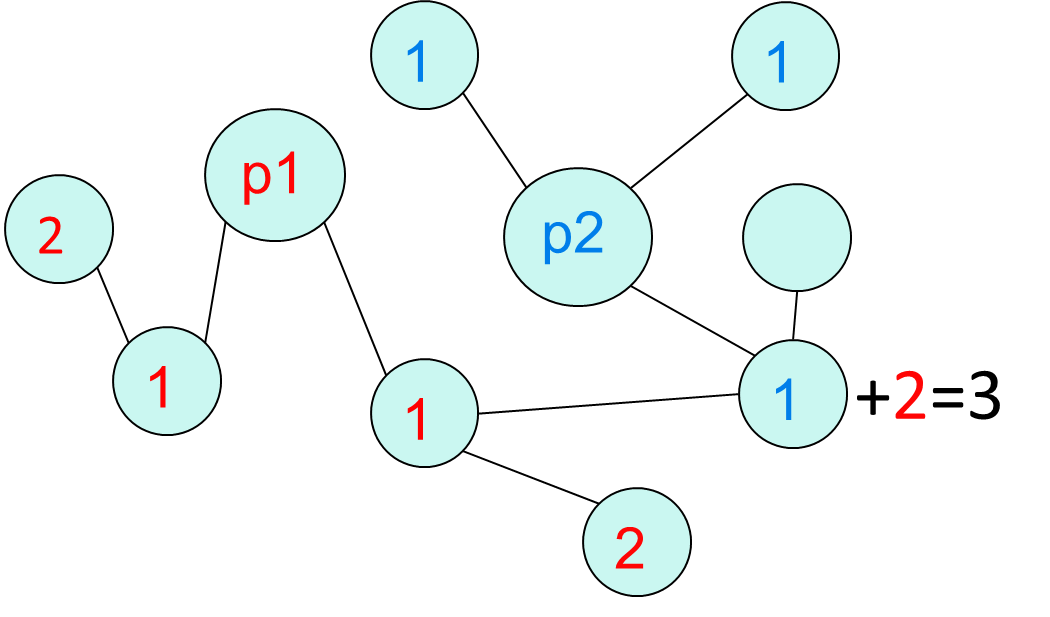
\includegraphics[width=0.5\textwidth]{res/q1.png}
\end{center}

\textbf{Solution:} Execute BFS from both $p_1$ and $p_2$.
Use a bit-array maintaining all the
visited vertices, to see if they have met
in the middle.

\end{frame}

%File: q2.tex
%Date: Wed Jun 25 00:16:23 2014 +0800
%Author: Yuxin Wu <ppwwyyxxc@gmail.com>

\section{Query 2}
\begin{frame}{Query 2}
Given $k$ and $d$, find top-$k$ tags with largest range. Here the
range of a tag $T$ in graph $G(V, E)$ is defined as the size of the
largest subgraph $G(V', E')$ s.t. $\forall v \in V ,v_d > d,  T \in v_t $.

\textbf{Solution:} First sort all the queries and vertices by $d$ in descending order.
Build an empty graph $G_0$ and incrementally insert sorted
vertices and their corresponding edges to $G_0$ .
  During the insertion, we maintain the top-$k$ largest connected
components for each tag using Union-Find Set. A query $q$ would
finish as soon as all vertices $v$ with $v_d>q_d$ are inserted.
\end{frame}

%File: q3.tex
%Date: Wed Jun 25 02:54:22 2014 +0800
%Author: Yuxin Wu <ppwwyyxxc@gmail.com>

\section{Query 3}
\begin{frame}{Query 3}
Given $k$ , $h$ , $p$ , where $p$ is used to define a subset $V′$ of $V$. Find
the top-$k$ pairs of vertex $(u, v)$ ordered by $|u_t \cap v_t|$, also
satisfying: $u, v \in V,  dist (u, v) \le h$.

\textbf{Solution:} Build an inverted
list for every tag $T$: $L(T) = $ a list of vertex $v \in V′ $where$ T \in v_t $.
This way, we can quickly find vertices in $V′$ sharing tags with a
given $v$ by counting \# of occurrences in inverted lists.
\end{frame}

%File: q4.tex
%Date: Wed Jun 25 05:38:40 2014 +0800
%Author: Yuxin Wu <ppwwyyxxc@gmail.com>

\section{Query 4}
\begin{frame}{Query 4}
  Given $k$ , $t$ , where $t$ is used to define a subgraph $G′$ of $G$, find
  the top-$k$ centralized vertex in $G′$. Here the centrality for a
  vertex $v$ in a graph $G(V, E)$ is defined as:

  \[ C(v) = \dfrac{r(v)^2}{(|V| - 1) S(v)},\]
    where $ r(v)$ is \# of vertex reachable from $v$ (exclusive),
 $ S(v) = \sum_{u\in V} dist(u, v) $ is very expensive to calculate.

\end{frame}

\begin{frame}{Framework}
  General framework to obtain top-$k$ centrality:
  \begin{enumerate}
    \item
      Estimate an upper bound of $C(v)$
      for each $v$ and maintain them with a max-heap.

    \item

      Iteratively pop the top element from the heap and calculate
      its actual value. If the actual value is still the largest in
      heap, then it's certainly the largest among all actual values
      of remaining element. Otherwise we insert this actual value
      back to the heap.
      \begin{center}
        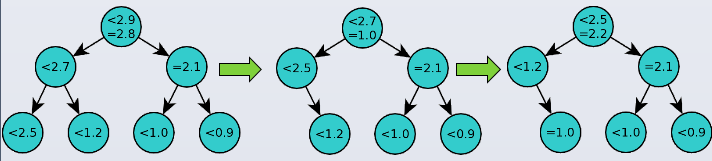
\includegraphics[width=0.9\textwidth]{res/heap.png}
      \end{center}
  \end{enumerate}

\end{frame}

\begin{frame}{Lower Bound of $ S(v)$}
  \[ S(v) \ge \sum_{dist(u, v) \le \ell}dist(u, v) + \sum_{dist(u,v)>\ell}(\ell + 1) \]

The first term is calculated by a BFS from $v$ with search depth
limited to $\ell$. The second term is obtained by counting.

To choose a proper $\ell$, we compare our current estimation of each
$S(v)$ to an approximation of $S(v)$ and increase $\ell$ when the mean-
square error is large. Since social networks have \textbf{small
  diameter(!)}, a small $\ell$ (3 or 4) is sufficient to guarantee a good
lower bound estimation of $S(v)$.

\end{frame}

\begin{frame}{Approximation of $ S(v)$}
Random sample a subset $ V_1$ of $ V$, and run a thorough BFS
on each of them, giving $ dist(u, v)$ for each $u \in V_1 $ and $ v \in V$. Then we
have:

\[ \forall v \in V, S(v) \approx \sum_{u\in V_1} dist(u, v)\dfrac{|V|}{|V_1|} \]

This is a highly accurate approximation, which gave an average
1$\sim$2\% error sampled with 0.1\% of $V$ in our experiments.

This approximation can also help with pruning: by calculating
actual centrality of the vertices with top-$(3k)$ approximated
centrality, we get $3k$ actual centrality that is very likely to
contain the actual top-$k$ centralities. Then the $k$th centrality
among the $3k$ results is a very good lower bound of the top-$k$ centrality.

\end{frame}

%File: trick.tex
%Date: Wed Jun 25 00:42:05 2014 +0800
%Author: Yuxin Wu <ppwwyyxxc@gmail.com>

\section{Others}
\begin{frame}{Other tricks}
  \begin{enumerate}

    \item Use mmap() to read data files faster.

    \item Implement a thread pool to utilize multi-core processors.

    \item Google's tcmalloc is faster to allocate memory.

    \item

      Another way of BFS in estimating lower bound in query 4
      is to use a bitset $ B_{\ell}(v)$ of length $ |V|$ whose $ u$th bit
      is set iff. $ dist(u, v) =\ell$. Then we have:
      \[ B_{\ell+1}(v)  = \neg B_{\ell}(v) \wedge (\vee_{(u, v) \in E}B_{\ell}(u))\]

      This search can be implemented using SIMD instructions.
  \end{enumerate}
\end{frame}




\begin{frame}{}
  \begin{center}
  \Huge Thanks!
\end{center}
\end{frame}

\end{document}

